% Options for packages loaded elsewhere
\PassOptionsToPackage{unicode}{hyperref}
\PassOptionsToPackage{hyphens}{url}
%
\documentclass[
]{article}
\usepackage{lmodern}
\usepackage{amssymb,amsmath}
\usepackage{ifxetex,ifluatex}
\ifnum 0\ifxetex 1\fi\ifluatex 1\fi=0 % if pdftex
  \usepackage[T1]{fontenc}
  \usepackage[utf8]{inputenc}
  \usepackage{textcomp} % provide euro and other symbols
\else % if luatex or xetex
  \usepackage{unicode-math}
  \defaultfontfeatures{Scale=MatchLowercase}
  \defaultfontfeatures[\rmfamily]{Ligatures=TeX,Scale=1}
\fi
% Use upquote if available, for straight quotes in verbatim environments
\IfFileExists{upquote.sty}{\usepackage{upquote}}{}
\IfFileExists{microtype.sty}{% use microtype if available
  \usepackage[]{microtype}
  \UseMicrotypeSet[protrusion]{basicmath} % disable protrusion for tt fonts
}{}
\makeatletter
\@ifundefined{KOMAClassName}{% if non-KOMA class
  \IfFileExists{parskip.sty}{%
    \usepackage{parskip}
  }{% else
    \setlength{\parindent}{0pt}
    \setlength{\parskip}{6pt plus 2pt minus 1pt}}
}{% if KOMA class
  \KOMAoptions{parskip=half}}
\makeatother
\usepackage{xcolor}
\IfFileExists{xurl.sty}{\usepackage{xurl}}{} % add URL line breaks if available
\IfFileExists{bookmark.sty}{\usepackage{bookmark}}{\usepackage{hyperref}}
\hypersetup{
  pdftitle={week3\_2.R},
  pdfauthor={danie},
  hidelinks,
  pdfcreator={LaTeX via pandoc}}
\urlstyle{same} % disable monospaced font for URLs
\usepackage[margin=1in]{geometry}
\usepackage{color}
\usepackage{fancyvrb}
\newcommand{\VerbBar}{|}
\newcommand{\VERB}{\Verb[commandchars=\\\{\}]}
\DefineVerbatimEnvironment{Highlighting}{Verbatim}{commandchars=\\\{\}}
% Add ',fontsize=\small' for more characters per line
\usepackage{framed}
\definecolor{shadecolor}{RGB}{248,248,248}
\newenvironment{Shaded}{\begin{snugshade}}{\end{snugshade}}
\newcommand{\AlertTok}[1]{\textcolor[rgb]{0.94,0.16,0.16}{#1}}
\newcommand{\AnnotationTok}[1]{\textcolor[rgb]{0.56,0.35,0.01}{\textbf{\textit{#1}}}}
\newcommand{\AttributeTok}[1]{\textcolor[rgb]{0.77,0.63,0.00}{#1}}
\newcommand{\BaseNTok}[1]{\textcolor[rgb]{0.00,0.00,0.81}{#1}}
\newcommand{\BuiltInTok}[1]{#1}
\newcommand{\CharTok}[1]{\textcolor[rgb]{0.31,0.60,0.02}{#1}}
\newcommand{\CommentTok}[1]{\textcolor[rgb]{0.56,0.35,0.01}{\textit{#1}}}
\newcommand{\CommentVarTok}[1]{\textcolor[rgb]{0.56,0.35,0.01}{\textbf{\textit{#1}}}}
\newcommand{\ConstantTok}[1]{\textcolor[rgb]{0.00,0.00,0.00}{#1}}
\newcommand{\ControlFlowTok}[1]{\textcolor[rgb]{0.13,0.29,0.53}{\textbf{#1}}}
\newcommand{\DataTypeTok}[1]{\textcolor[rgb]{0.13,0.29,0.53}{#1}}
\newcommand{\DecValTok}[1]{\textcolor[rgb]{0.00,0.00,0.81}{#1}}
\newcommand{\DocumentationTok}[1]{\textcolor[rgb]{0.56,0.35,0.01}{\textbf{\textit{#1}}}}
\newcommand{\ErrorTok}[1]{\textcolor[rgb]{0.64,0.00,0.00}{\textbf{#1}}}
\newcommand{\ExtensionTok}[1]{#1}
\newcommand{\FloatTok}[1]{\textcolor[rgb]{0.00,0.00,0.81}{#1}}
\newcommand{\FunctionTok}[1]{\textcolor[rgb]{0.00,0.00,0.00}{#1}}
\newcommand{\ImportTok}[1]{#1}
\newcommand{\InformationTok}[1]{\textcolor[rgb]{0.56,0.35,0.01}{\textbf{\textit{#1}}}}
\newcommand{\KeywordTok}[1]{\textcolor[rgb]{0.13,0.29,0.53}{\textbf{#1}}}
\newcommand{\NormalTok}[1]{#1}
\newcommand{\OperatorTok}[1]{\textcolor[rgb]{0.81,0.36,0.00}{\textbf{#1}}}
\newcommand{\OtherTok}[1]{\textcolor[rgb]{0.56,0.35,0.01}{#1}}
\newcommand{\PreprocessorTok}[1]{\textcolor[rgb]{0.56,0.35,0.01}{\textit{#1}}}
\newcommand{\RegionMarkerTok}[1]{#1}
\newcommand{\SpecialCharTok}[1]{\textcolor[rgb]{0.00,0.00,0.00}{#1}}
\newcommand{\SpecialStringTok}[1]{\textcolor[rgb]{0.31,0.60,0.02}{#1}}
\newcommand{\StringTok}[1]{\textcolor[rgb]{0.31,0.60,0.02}{#1}}
\newcommand{\VariableTok}[1]{\textcolor[rgb]{0.00,0.00,0.00}{#1}}
\newcommand{\VerbatimStringTok}[1]{\textcolor[rgb]{0.31,0.60,0.02}{#1}}
\newcommand{\WarningTok}[1]{\textcolor[rgb]{0.56,0.35,0.01}{\textbf{\textit{#1}}}}
\usepackage{graphicx,grffile}
\makeatletter
\def\maxwidth{\ifdim\Gin@nat@width>\linewidth\linewidth\else\Gin@nat@width\fi}
\def\maxheight{\ifdim\Gin@nat@height>\textheight\textheight\else\Gin@nat@height\fi}
\makeatother
% Scale images if necessary, so that they will not overflow the page
% margins by default, and it is still possible to overwrite the defaults
% using explicit options in \includegraphics[width, height, ...]{}
\setkeys{Gin}{width=\maxwidth,height=\maxheight,keepaspectratio}
% Set default figure placement to htbp
\makeatletter
\def\fps@figure{htbp}
\makeatother
\setlength{\emergencystretch}{3em} % prevent overfull lines
\providecommand{\tightlist}{%
  \setlength{\itemsep}{0pt}\setlength{\parskip}{0pt}}
\setcounter{secnumdepth}{-\maxdimen} % remove section numbering

\title{week3\_2.R}
\author{danie}
\date{2021-06-24}

\begin{document}
\maketitle

\begin{Shaded}
\begin{Highlighting}[]
\KeywordTok{library}\NormalTok{(readr)}
\KeywordTok{library}\NormalTok{(readxl)}
\KeywordTok{library}\NormalTok{(dplyr)}
\end{Highlighting}
\end{Shaded}

\begin{verbatim}
## 
## Attaching package: 'dplyr'
\end{verbatim}

\begin{verbatim}
## The following objects are masked from 'package:stats':
## 
##     filter, lag
\end{verbatim}

\begin{verbatim}
## The following objects are masked from 'package:base':
## 
##     intersect, setdiff, setequal, union
\end{verbatim}

\begin{Shaded}
\begin{Highlighting}[]
\KeywordTok{library}\NormalTok{(tidyr)}
\KeywordTok{library}\NormalTok{(ggplot2)}
\KeywordTok{library}\NormalTok{(Hmisc)}
\end{Highlighting}
\end{Shaded}

\begin{verbatim}
## Loading required package: lattice
\end{verbatim}

\begin{verbatim}
## Loading required package: survival
\end{verbatim}

\begin{verbatim}
## Loading required package: Formula
\end{verbatim}

\begin{verbatim}
## 
## Attaching package: 'Hmisc'
\end{verbatim}

\begin{verbatim}
## The following objects are masked from 'package:dplyr':
## 
##     src, summarize
\end{verbatim}

\begin{verbatim}
## The following objects are masked from 'package:base':
## 
##     format.pval, units
\end{verbatim}

\begin{Shaded}
\begin{Highlighting}[]
\KeywordTok{library}\NormalTok{(PerformanceAnalytics)}
\end{Highlighting}
\end{Shaded}

\begin{verbatim}
## Loading required package: xts
\end{verbatim}

\begin{verbatim}
## Loading required package: zoo
\end{verbatim}

\begin{verbatim}
## 
## Attaching package: 'zoo'
\end{verbatim}

\begin{verbatim}
## The following objects are masked from 'package:base':
## 
##     as.Date, as.Date.numeric
\end{verbatim}

\begin{verbatim}
## 
## Attaching package: 'xts'
\end{verbatim}

\begin{verbatim}
## The following objects are masked from 'package:dplyr':
## 
##     first, last
\end{verbatim}

\begin{verbatim}
## 
## Attaching package: 'PerformanceAnalytics'
\end{verbatim}

\begin{verbatim}
## The following object is masked from 'package:graphics':
## 
##     legend
\end{verbatim}

\begin{Shaded}
\begin{Highlighting}[]
\KeywordTok{library}\NormalTok{(treemap)}
\KeywordTok{library}\NormalTok{(areaplot)}

\NormalTok{unemployment <-}\StringTok{ }\KeywordTok{read_csv}\NormalTok{(}\StringTok{"C:/Users/danie/OneDrive/DSC-640/week3_4/unemployement-rate-1948-2010.csv"}\NormalTok{)}
\end{Highlighting}
\end{Shaded}

\begin{verbatim}
## 
## -- Column specification --------------------------------------------------------
## cols(
##   `Series id` = col_character(),
##   Year = col_double(),
##   Period = col_character(),
##   Value = col_double()
## )
\end{verbatim}

\begin{Shaded}
\begin{Highlighting}[]
\NormalTok{us_postage <-}\StringTok{ }\KeywordTok{read_excel}\NormalTok{(}\StringTok{"C:/Users/danie/OneDrive/DSC-640/week3_4/us-postage.xlsm"}\NormalTok{)}
\NormalTok{world_population <-}\StringTok{ }\KeywordTok{read_excel}\NormalTok{(}\StringTok{"C:/Users/danie/OneDrive/DSC-640/week3_4/world-population.xlsm"}\NormalTok{)}

\CommentTok{# Label for tree map}
\NormalTok{us_postage[}\StringTok{"label"}\NormalTok{] <-}\StringTok{ }\KeywordTok{paste}\NormalTok{(us_postage}\OperatorTok{$}\NormalTok{Year, }\StringTok{":"}\NormalTok{, us_postage}\OperatorTok{$}\NormalTok{Price)}
\NormalTok{us_postage[}\StringTok{"label"}\NormalTok{]}
\end{Highlighting}
\end{Shaded}

\begin{verbatim}
## # A tibble: 10 x 1
##    label      
##    <chr>      
##  1 1991 : 0.29
##  2 1995 : 0.32
##  3 1999 : 0.33
##  4 2001 : 0.34
##  5 2002 : 0.37
##  6 2006 : 0.39
##  7 2007 : 0.41
##  8 2008 : 0.42
##  9 2009 : 0.44
## 10 2010 : 0.44
\end{verbatim}

\begin{Shaded}
\begin{Highlighting}[]
\NormalTok{us_postage}
\end{Highlighting}
\end{Shaded}

\begin{verbatim}
## # A tibble: 10 x 3
##     Year Price label      
##    <dbl> <dbl> <chr>      
##  1  1991  0.29 1991 : 0.29
##  2  1995  0.32 1995 : 0.32
##  3  1999  0.33 1999 : 0.33
##  4  2001  0.34 2001 : 0.34
##  5  2002  0.37 2002 : 0.37
##  6  2006  0.39 2006 : 0.39
##  7  2007  0.41 2007 : 0.41
##  8  2008  0.42 2008 : 0.42
##  9  2009  0.44 2009 : 0.44
## 10  2010  0.44 2010 : 0.44
\end{verbatim}

\begin{Shaded}
\begin{Highlighting}[]
\CommentTok{# Creating Tree Map}
\KeywordTok{treemap}\NormalTok{(us_postage,}\DataTypeTok{index =} \KeywordTok{c}\NormalTok{(}\StringTok{"label"}\NormalTok{) ,}\DataTypeTok{vSize =}\StringTok{"Price"}\NormalTok{,}\DataTypeTok{title =} \StringTok{"Price vs Year"}\NormalTok{)}
\end{Highlighting}
\end{Shaded}

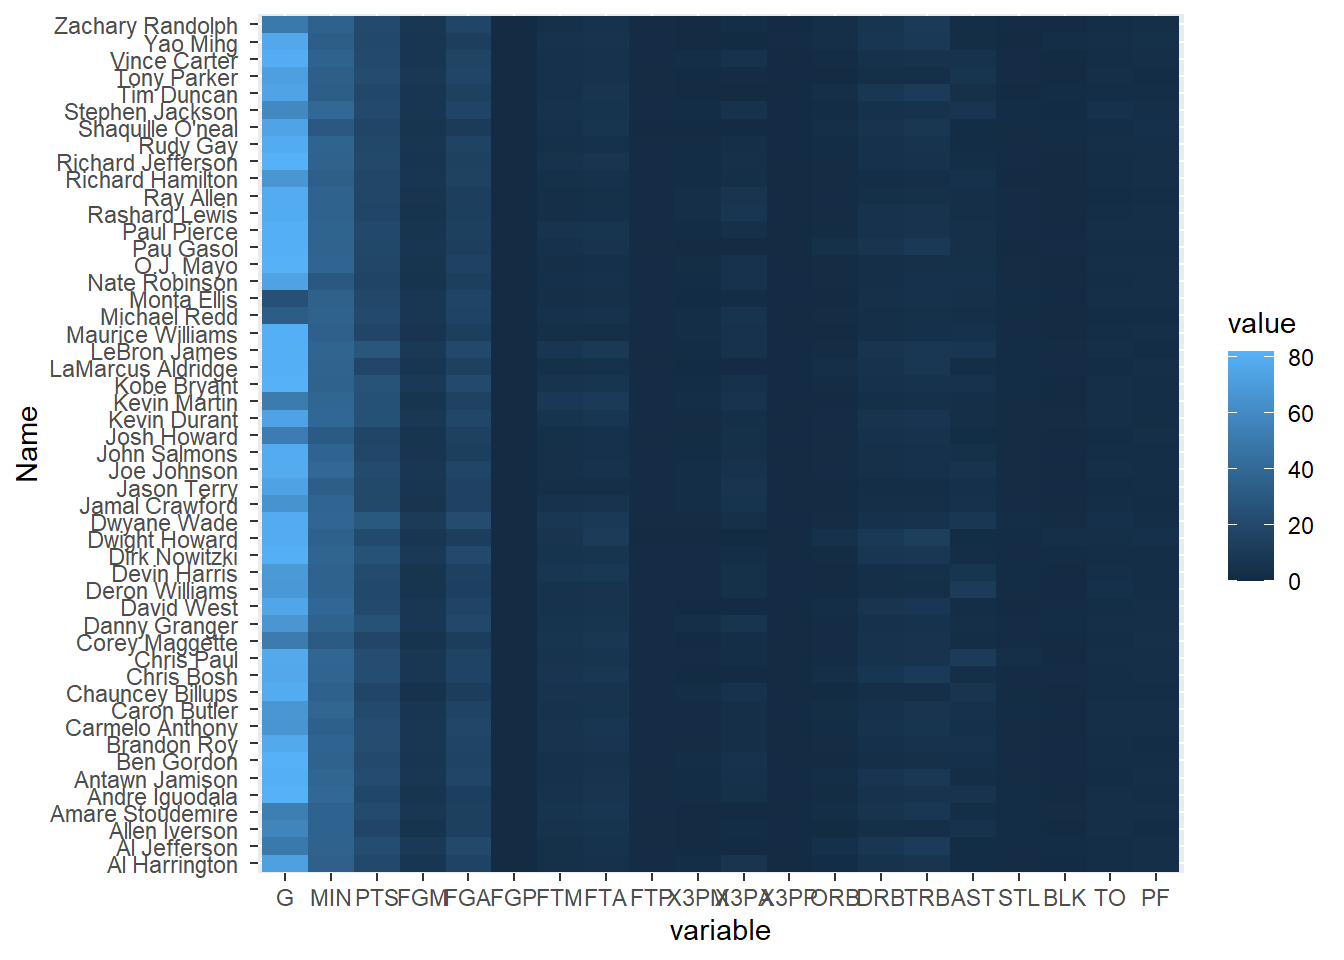
\includegraphics{week3_2_files/figure-latex/unnamed-chunk-1-1.pdf}

\begin{Shaded}
\begin{Highlighting}[]
\CommentTok{# create area map}
\KeywordTok{ggplot}\NormalTok{(world_population, }\KeywordTok{aes}\NormalTok{(}\DataTypeTok{x=}\NormalTok{Year, }\DataTypeTok{y=}\NormalTok{Population))}\OperatorTok{+}\KeywordTok{geom_area}\NormalTok{(}\DataTypeTok{fill=}\StringTok{'#F9c19918'}\NormalTok{,}\DataTypeTok{alpha=}\DecValTok{2}\NormalTok{)}
\end{Highlighting}
\end{Shaded}

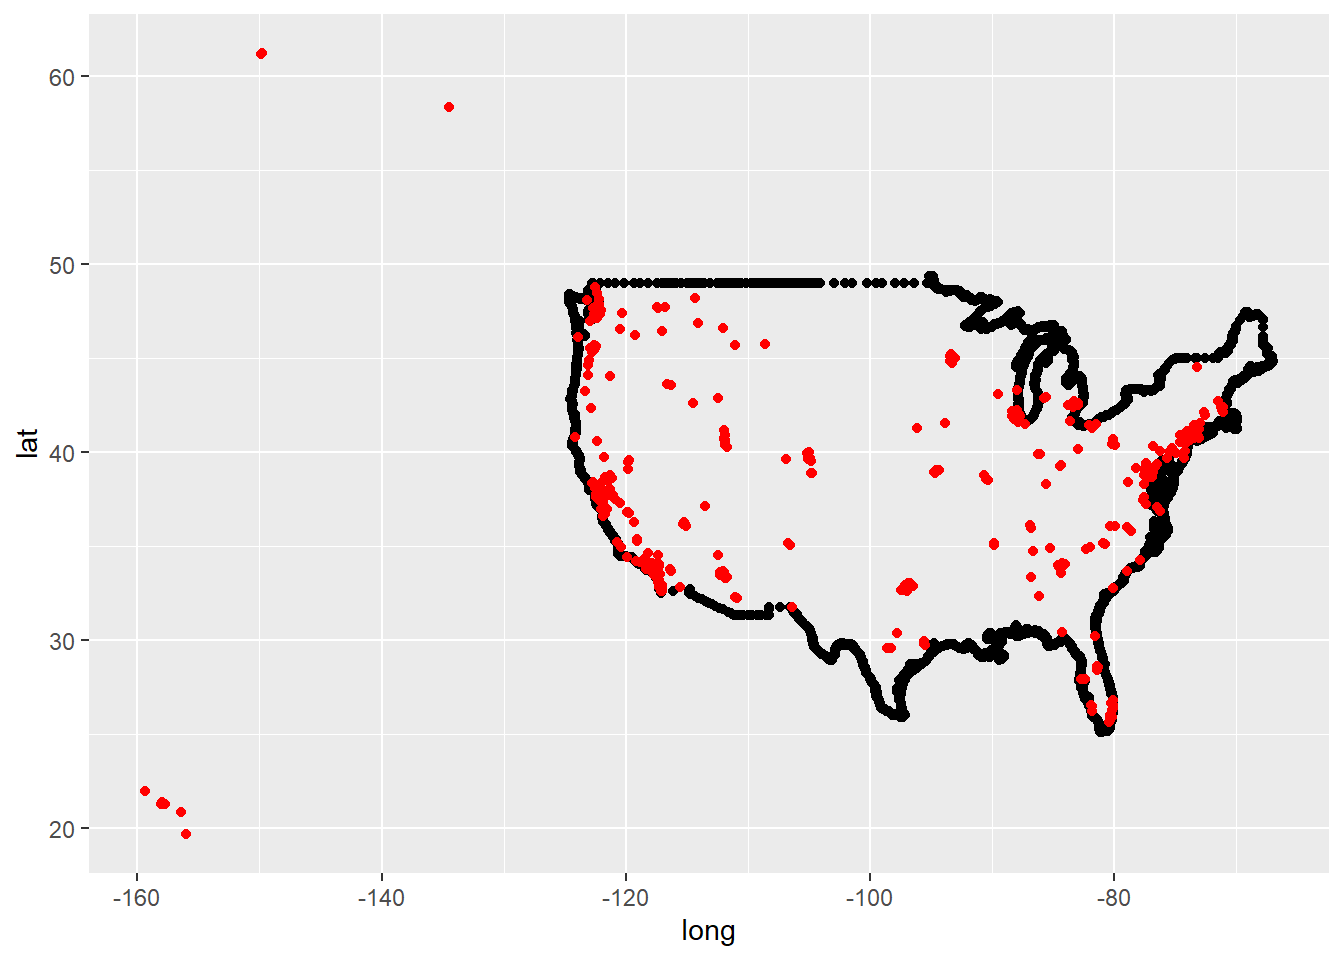
\includegraphics{week3_2_files/figure-latex/unnamed-chunk-1-2.pdf}

\begin{Shaded}
\begin{Highlighting}[]
\CommentTok{# Stacked area chart}
\KeywordTok{ggplot}\NormalTok{(unemployment, }\KeywordTok{aes}\NormalTok{(}\DataTypeTok{x=}\NormalTok{Year, }\DataTypeTok{y=}\NormalTok{Value, }\DataTypeTok{fill=}\NormalTok{Period )) }\OperatorTok{+}\StringTok{ }
\StringTok{  }\KeywordTok{geom_area}\NormalTok{()}
\end{Highlighting}
\end{Shaded}

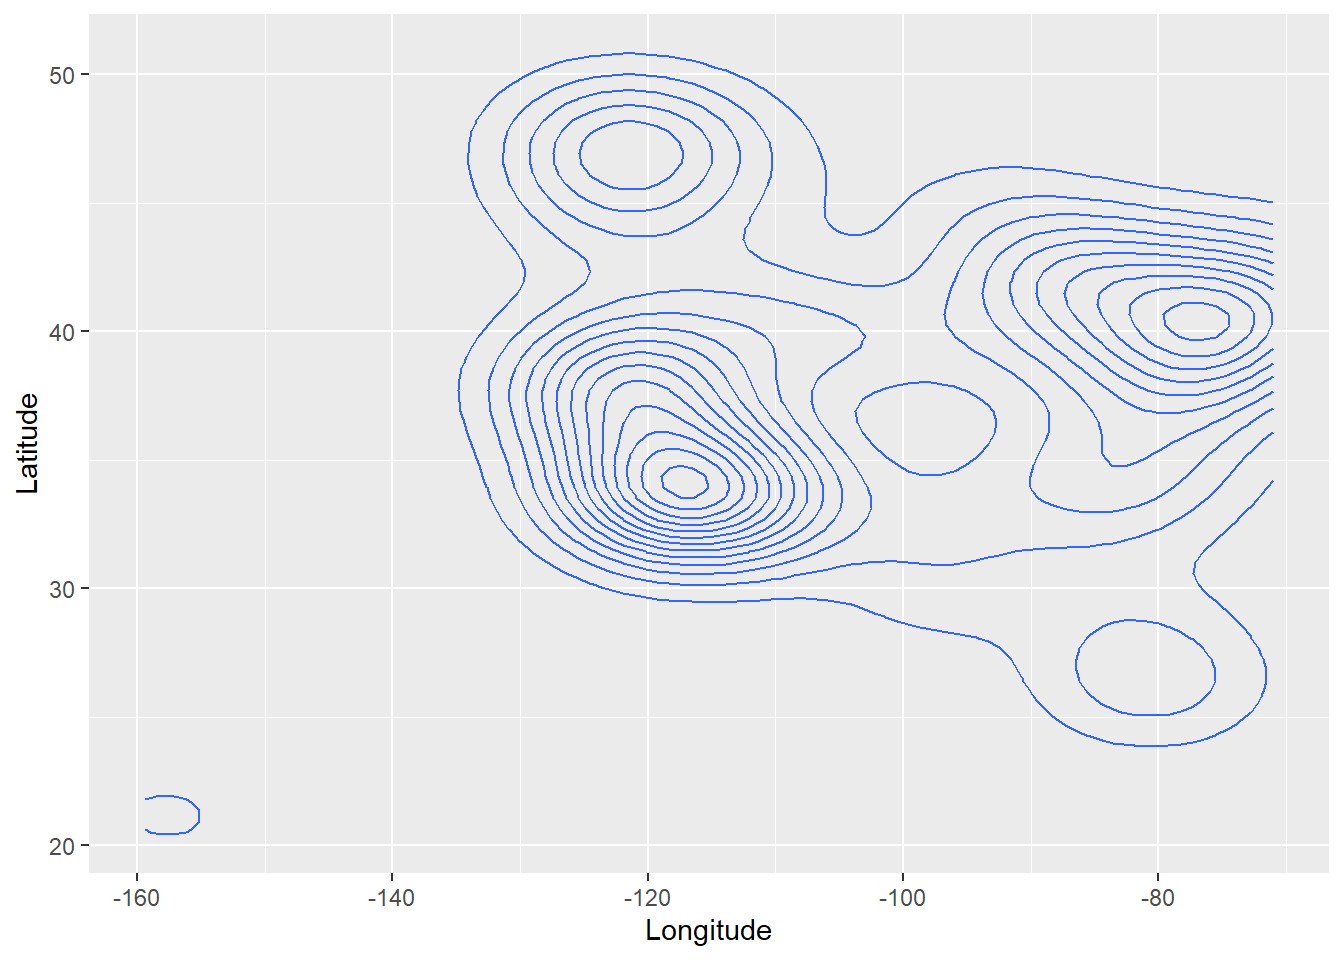
\includegraphics{week3_2_files/figure-latex/unnamed-chunk-1-3.pdf}

\begin{Shaded}
\begin{Highlighting}[]
\CommentTok{# Step Chart}
\KeywordTok{ggplot}\NormalTok{(unemployment, }\KeywordTok{aes}\NormalTok{(Year,Value)) }\OperatorTok{+}\StringTok{ }\KeywordTok{geom_step}\NormalTok{() }\OperatorTok{+}\StringTok{ }\CommentTok{#Ploting}
\StringTok{  }\KeywordTok{scale_y_continuous}\NormalTok{(}\DataTypeTok{name=} \StringTok{"Year"}\NormalTok{) }\OperatorTok{+}
\StringTok{  }\KeywordTok{scale_x_continuous}\NormalTok{(}\DataTypeTok{name=} \StringTok{"Value"}\NormalTok{)}
\end{Highlighting}
\end{Shaded}

\includegraphics{week3_2_files/figure-latex/unnamed-chunk-1-4.pdf}

\end{document}
